\section{Results and Discussion}
\begin{table}
	\caption{Precision, recall, and efficiency comparison}
	\centering
	%\fontsize{8pt}{9.2pt}\selectfont
	%\setlength\tabcolsep{2px}
	\begin{threeparttable}
		\bgroup
		%\def\arraystretch{1.2}
		\begin{tabular}{l r r c}
			\toprule
											& \textbf{VIPS}		& \textbf{Cortex}  & \textbf{Significance} 	\\
			\toprule
			Precision          				& 32.1\%            & \textbf{50.1}\%  & $t_{score} = $ 5.15    \\
											& 					& 				   & $p < 0.00001$ 			\\
			relative improvement          	& ---               & 156.1\%          & \ 						\\
			\midrule 
			Recall         					& 13.7\%            & \textbf{38.8}\%  & $t_{score} = $ 5.29    \\
											& 					& 				   & $p < 0.00001$ 			\\
			
			relative improvement         	& ---               & 283.2\%          & \ 						\\
			\midrule
			F-measure         				& 15.7\%            & \textbf{39.1}\%  & $t_{score} = $ 6.67    \\
											& 					& 				   & $p < 0.00001$ 			\\

			relative improvement          	& ---               & 249.0\%          & \   					\\
			\midrule
			Efficiency (seconds)  			& 57.3 s            & \textbf{0.694} s & $t_{score} = $ 7.76    \\
											& 					& 				   & $p < 0.00001$ 			\\
			relative improvement          	& ---               & 8,256.5\%        & \   					\\
			\bottomrule

		\end{tabular}
		\egroup
	\end{threeparttable}
	\label{tbl:results-summary}
\end{table}

\begin{figure}
    \centering
    {%
    \setlength{\fboxsep}{0pt}%
    \setlength{\fboxrule}{1pt}%
    \fbox{
\includegraphics[trim=0 230 475 0,clip,scale=0.31]{figures/results-and-discussion/ground-truth.png}}
    }%
    \\Ground truth\\ \ \\
    {%
    \setlength{\fboxsep}{0pt}%
    \setlength{\fboxrule}{1pt}%
    \fbox{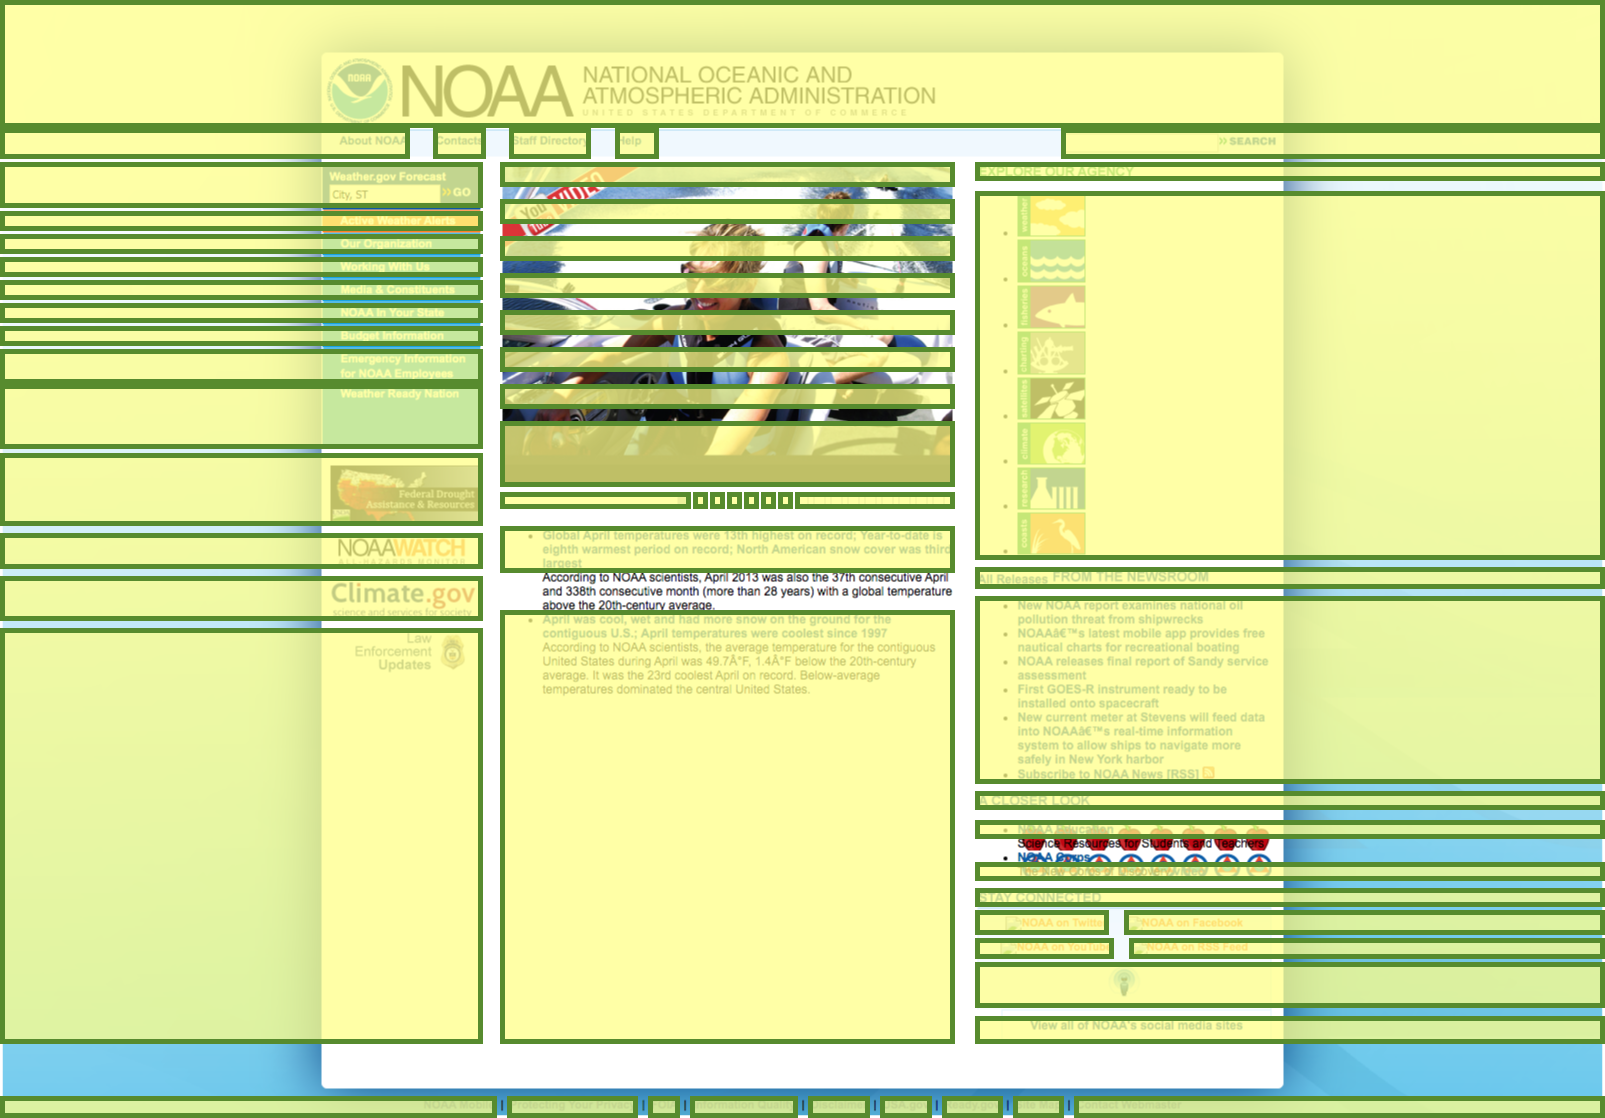
\includegraphics[trim=0 230 475 0,clip,scale=0.31]{figures/results-and-discussion/vips-output.png}}
    }%
    \\VIPS segmentation\\ \ \\
    {%
    \setlength{\fboxsep}{0pt}%
    \setlength{\fboxrule}{1pt}%
    \fbox{
\includegraphics[trim=0 230 475 0,clip,scale=0.31]{figures/results-and-discussion/cortex-output.png}}
    }%
    \\Cortex segmentation
    \caption{Comparison of ground truth segments to the 
    segments generated by VIPS and Cortex. 
    Each yellow highlighted rectangle represents a segment. }
    \label{fig:output-comparison}
\end{figure}

\begin{figure}
    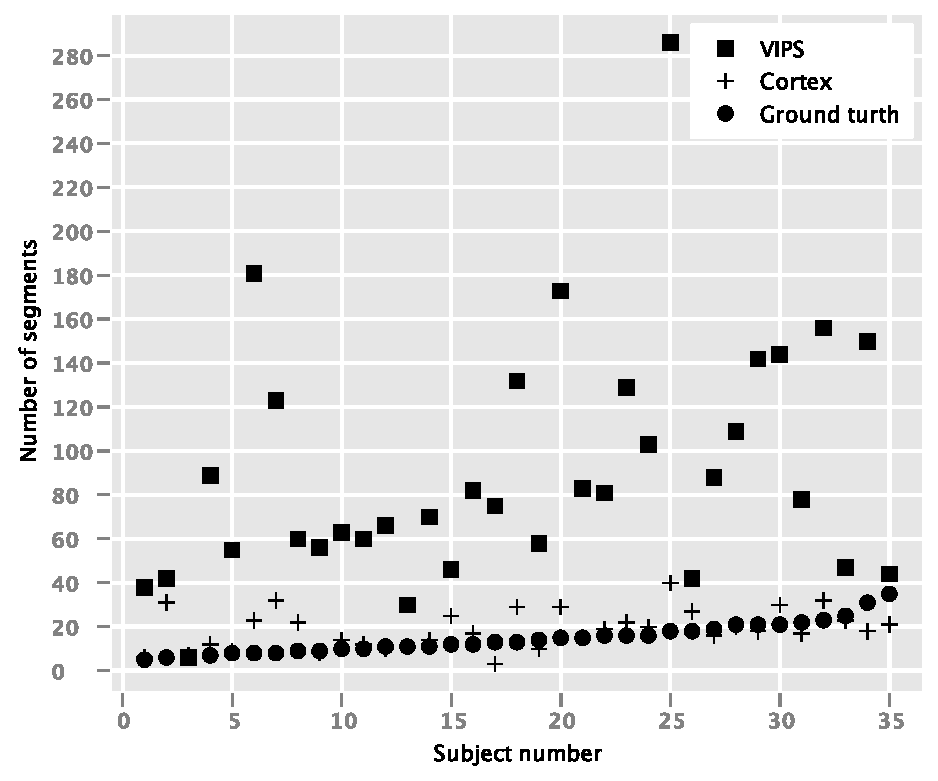
\includegraphics[trim=0 0 0 0,clip,scale=0.56]{figures/results-and-discussion/number-of-segments-fig.pdf}
    \caption{Number of segments generated by VIPS and Cortex, compared to ground truth.}
    \label{fig:number-of-segments}
\end{figure}


\Cref{tbl:results-summary} shows a summary of
the precision, recall, and efficiency evaluation. 
The first column shows the variable being measured,
in both its absolute value as well as relative improvement percentage
relative to baseline.
The second and third columns show the
measured evaluation average for both VIPS and Cortex,
respectively, across all subjects.
Finally, the third column tests for statistical significance
using Welch's unequal variances t-test. 
\toolname's average precision was 50.1\%
compared to 32.1\% for VIPS, showing an improvement of 156.1\%.
The result was highly statistically significant,
with a t-score of 5.15 and $p <$ 0.00001.
The recall, F-measure, and runtime
also showed an improvement of 283.2\%, 249\%, and 8,256.5\%, 
respectively, relative to VIPS.
All evaluation improvements were statistically significant with $p <$ 0.00001.

We now investigate these results in more detail
in order to understand the reasons behind
the measured differences in evaluation outcomes.
We begin by showing how the output of segmentation looks like.
\Cref{fig:output-comparison} shows the segments generated
by VIPS and \toolname for one of the evaluation subjects.
For reference, the ground truth segments for that subject
are also shown in the figure.
Each segment is represented by a rectangle
with a yellow highlight and a green border.

We make a number of observations
from the comparison of the two outputs.
First, from a big picture perspective,
it can be observed that the \toolname
output is more similar to ground truth,
compared to VIPS' output.
That is, the overall arrangement, count, and size of segments
from \toolname has better resemblance to ground truth.
This illustrates an example of the reason behind the measured
evaluation improvements for \toolname.
In order to better understand these improvements, we 
examine how VIPS is performing 
and then contrast how \toolname generates better results.
We first observe that the precision of VIPS is relatively low,
as can be seen from the typically very large sizes of the generated segments.
VIPS does not create precise segments that closely match the ground truth.
Rather, it has a tendency of oversegmentation, where almost
every element ends up being in its own segment.
\Cref{fig:number-of-segments} illustrates this behavior,
where the number of segments generated by both VIPS and \toolname
are plotted for all subjects. Note how VIPS has a tendency of generating
significantly more segments than necessary.
This can be seen, for example, in the VIPS output in \Cref{fig:output-comparison},
where there are many segments over the central image element,
and over the small buttons under it.
This might be attributed to VIPS' iterative nature
and its lack of accurate definition of visual elements,
therefore increasing the likelihood that more segments are generated.
Contrast this with the one-step approach used in \toolname.
The segments are generated in a non-iterative fashion,
and the segments originate from abstract visual objects as opposed to 
the entire DOM node set.
The final number of segments would therefore tend 
to be relatively small compared to VIPS,
which reduces the potential for false positives
and results in a relatively higher precision.

\begin{figure}
    \centering
    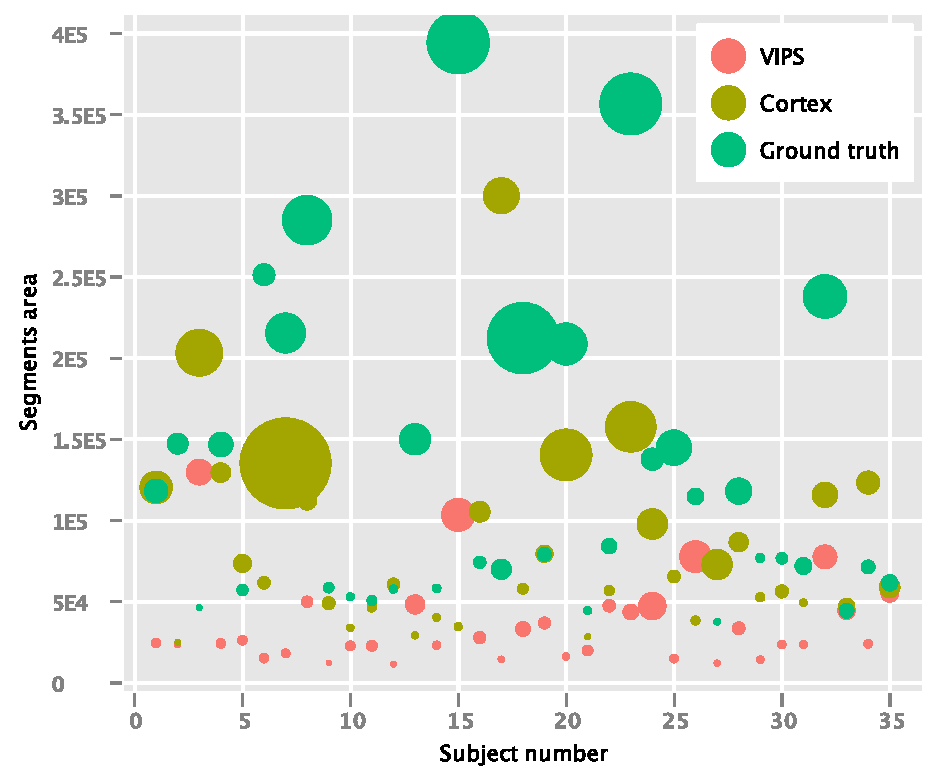
\includegraphics[trim=0 0 0 0,clip,scale=0.56]{figures/results-and-discussion/segment-area-plot.pdf}
    \caption{Generated segment areas of VIPS and Cortex compared to ground truth.
    Y value is the average segment area and bubble size is the standard deviation.}
    \label{fig:segment-area}
\end{figure}

VIPS also tends to include more elements in a segment,
resulting in larger segments and lower precision.
For instance, in \Cref{fig:output-comparison} note how the VIPS segments
of the left menu sidebar include the entire row,
resulting in a segment that includes non-visible parent elements that have greater
areas but are not visually present on the screen.
This might be attributed to VIPS' top-down approach,
where it starts from the whole page as one segment,
then iteratively divides it into smaller segments.
The final segments would therefore generally be
expected to have a tendency to be large, because the starting segment
is of maximum size (i.e., the whole page).

However, the same iterative behavior in VIPS would also equally
generate very small segments when the iteration stopping condition is not met.
This can be seen, for instance, in the VIPS output in \Cref{fig:output-comparison}
for the small button under the central image, and also the four small squares
around the top menu bar items.
\Cref{fig:segment-area} illustrates this behavior.
The figure shows a bubble plot of the segment areas for each subject.
The y-value of each bubble indicates the average segment area for that subject,
and the bubble size indicate the standard deviation of areas.
Note how \toolname generates segments that have more similar areas and distribution
as the ground truth, compared to VIPS, where the segments are mainly located
at the bottom of the plot.

Contrast this with the non-iterative approach used in \toolname.
Here we start from small leaf nodes, and form segments
by merging. As there is no stopping condition to reach,
and therefore no continuous sub-division of segments is performed,
the final segments can therefore be expected
to be on the larger end of the spectrum.
This behavior, combined with the small number of generated segments
and better overlap with ground truth,
yields a relatively higher precision for \toolname.

However, the precision and recall of \toolname,
while relatively high, is still not ideal.
We attribute this to the feature selection and the clustering process.
\toolname has a tendency, as expected, to create different segments where there is
strong and pronounced variations in color. But this sometimes leads to oversegmentation.
For instance, in \Cref{fig:output-comparison} compare the \toolname segment
over the left menu sidebar with that in ground truth.
In the ground truth,
the top most part of the sidebar has a search field,
followed by an orange menu item,
followed by the rest of the menu.
While in ground truth these are all correctly identified as one segment,
\toolname identifies each of these three parts as their own separate segments
due to very pronounced color style differences.
The same behavior can be observed in the top most segment of ground truth.
While the top most area of ground truth has a separate logo and brand segment,
and another top menu segment,
these two parts are considered one segment in the \toolname output.

\header{Threats to validity}
To mitigate potential selection bias,
we selected a random set of subjects as described in \Cref{sec:rq-effectiveness}.
Furthermore, the subjects are diverse and complex enough to be
representative of real-world web pages,
mitigating threats to the external validity of the study by making the results generalizable.
To mitigate the experimenter-bias internal threat,
we use ground truth data that is publicly available and has been collected and labeled
by an external third-party.
Furthermore, we conduct statistical significance testing
to ensure the observed outcomes are significant.

\section{Related Work}
We already discussed some of the related work on page segmentation in \autoref{sec:background}.
Here we focus on techniques that
analyze web pages from a visual perspective.
An advantage of visual analysis approaches is that
they tend to better capture what an end user would perceive.
Choudhary et al.~\cite{choudhary2012crosscheck} propose
an approach that detects cross-browser compatibility
by examining visual differences between the same page running in multiple browsers.
Bajammal et al.~\cite{canvas_icst2018} propose an approach
to analyze and test web canvas element through visual
inference of the state of the canvas and its objects,
and allowing canvas elements to be testable using common DOM testing approaches.
Stocco et al.~\cite{2018-Stocco-FSE} employ computer vision techniques
 for visual-based web test repair and migrating DOM-based tests to visual tests.
Burg et al.~\cite{burg2015explaining} present a tool that helps
developers understand the behavior of web apps.
It allows developers to specify which element they are interested in,
then tracks that element for any visual changes and the corresponding code changes.
In contrast to our work,
none of these studies aims to automatically generate segments from a web page.


\section{Conclusions}

Web page segmentation is the process of extracting
sets of cohesive elements from a web page.
It has been used in various applications,
such as cross-browser testing,
mobile layout bugs testing and repair,
security testing, and crawling optimization.
However, existing segmentation approaches,
such as DOM-based, text-based, or vision-based segmentation,
have a number of drawbacks that reduce their accuracy.
In this paper, we proposed a novel visual segmentation approach.
Unlike existing state-of-the-art techniques,
which are mainly DOM-based with a few visual attributes,
our approach performs an extensive visual analysis that examines
the overall visual structure and layout of the page, 
and therefore more faithfully captures the visual structure of the page as perceived by a human user. 
While our approach is mainly visual in nature,
it also combines aspects of both DOM-based and visual-based segmentation
in a fashion that aims to minimize the drawbacks of each segmentation technique.
Furthermore, the approach is parameter-free,
requiring no thresholds for its operation and therefore
reduces the manual effort required and
makes the accuracy of the approach
independent of manual parameter tuning. 
We implemented our approach in a tool called \toolname,
and evaluated its effectiveness and efficiency of
segmenting real-world web pages. 
It achieved an average of 156\% improvement in precision
relative to state-of-the-art, 283\% improvement in recall, 
and a 249\% improvement in F-measure.
